
In this section we present the results of a controlled experiment in
which we injected bugs into \moss\ \cite{Schleimer:2003:WLA}, a widely
used plagiarism detection service.  A primary goal of this experiment
was to see whether our algorithm was effective at finding most or all
bugs in an application; thus it was necessary to know the set of bugs
we were looking for.  Both \moss\ source code and bug logs were
available to us, and so we could easily reproduce historical bugs.

We briefly describe the nine bugs we added to \moss.  As discussed in
\Autoref{sec:introduction}, these bugs vary from low-level crashing
bugs to high-level logic bugs that simply produce incorrect output.
Except where noted, these are all bugs that originally occurred in
\moss.
\begin{enumerate}
\item We reintroduced a bug that causes the number of
lines in C-style multi-line comments to be counted incorrectly.  This bug causes incorrect output
in certain circumstances: an option to
match comments must be on (normally \moss\ ignores comments)
and there must be matching multi-line comments that affect the output.

\item We removed a check for a
null {\tt FILE} pointer.  This is not originally a \moss\ bug; it is exactly analogous to the {\tt ccrypt} bug (see \Autoref{sec:revisited}).

\item We removed an array bounds update
in the routine for loading preprocessed data from disk. The
program behaves normally unless the function is called a second time,
in which case previously loaded data may be partially overwritten.
This bug has unpredictable effects and
was particularly difficult to find originally.

\item We removed a size check that prevents users from supplying command-line arguments
that could cause the program to overrun the bounds of an array.

\item For historical reasons, \moss\ handles Lisp programs differently
from all other languages.  We removed a end-of-list check in the Lisp-specific
code.

\item For efficiency \moss\ preallocates a large area of memory for its primary data structure.
When this area of memory is filled, the program should fail
gracefully.  We removed an out-of-memory check. 

\item \moss\ has a routine that scans an array for multiple copies of a data value.
We removed the limit check that prevents the code from searching past the end of the array.  
This bug did not occur in \moss; it is intended to be a more frequently occurring version of bug 8.

\item  A buffer overrun, this bug was never known to have caused a failure in \moss. It
was discovered originally by a code review.

\item This bug is a variant of bug 4, but involves a different command-line argument and
a different array.
\end{enumerate}

In summary, six of the nine bugs were originally bugs in \moss, two are variants on \moss bugs, and one
is a port of the {\tt ccrypt} bug.  The bugs
range from typical C coding errors (e.g., \texttt{NULL} pointer dereferences
and array overruns) to high-level violations of a system's internal
invariants (e.g., bugs 1 and 3).

To measure the accuracy of our techniques we logged 
when each bug was triggered.  Of course, this logging 
code was excluded from the sampling instrumentation.
To determine whether a run produced correct output we compared it against a run
of the reference version of \moss.  As discussed in \Autoref{sec:introduction},
in practice the labeling of runs as successful or failed is done by either detecting
crashes, internal assertion failures, or (speculatively) by direct user feedback that the output
of the program appears incorrect.  Our use of a reference version in this experiment made
it possible for us to label large numbers of runs automatically.

Table~\ref{tab:exps} shows that \moss\ has over 200,000 instrumented predicates,
and {\tt Rhythmbox} has over 800,000.
The reader may wonder whether it is practical to actually generate a report on
800,000 predicates on a client machine and then upload it to a central
server for analysis.  The answer is definitely yes.  Recall
that the predicates are synthesized from about half as many counters.
The counters are mostly zeroes and so compress extremely well,
resulting in uploaded files in the range of 10-50Kbytes.

As can be seen in Table~\ref{tab:exps}, the branches and returns schemes
resulted in short reports.  We again used correlations between predicates to help us navigate
the scalar-pairs report.

We briefly summarize the results.
The algorithm identified a highly-ranked cause that would be useful to a programmer
for six of the nine bugs.  For the two other bugs,
one (bug 7) occurred in our experiment but never caused
the program to crash or produce incorrect output; the other (bug 8) was never
triggered at all.  There is no way our algorithm can find causes of bugs that do not
occur, but recall that part of our purpose in sampling user executions
is to get an accurate picture of the most important bugs. It is consistent with
this goal that if a bug never causes a problem, it is not only not worth fixing,
it is not even worth reporting.  The remaining bug had a strong predictor in the reports,
but being a less important bug it was not highly ranked until other, higher-ranked
bugs were fixed, at which point its strongest predictor became highly ranked.

Both the branches and returns reports are quite short and most any sort order would be
reasonable.  Here we show the top six predicates, sorted in decreasing order of the probability
of the program failing when the predicate is true:
%%
\begin{verbatim}
Predicate      Context    Increase   Failure    Bug #
strcmp(s,"lisp") == 0  
               0.19       0.81       1.00       5
*pstart + numpassages > pmax - 1 
               0.53       0.47       1.00       6
config.match_comment != 0
               0.14       0.83       0.97       1
strmp(argv[i],"-p") == 0
               0.14       0.83       0.97       6
strmp(argv[i],"-s") == 0
               0.11       0.43       0.53       2
config.dbfile != NULL
               0.03       0.47       0.50       2
\end{verbatim}
We have added the last column by hand to show the bug each predicate indicates.  In
each case these predicates give a very strong hint to the programmer about the conditions
under which failure will occur.  We describe each briefly, in order.


The first predicate marks the line where the decision is made about
whether a Lisp program is being processed or not; the program always
fails for Lisp inputs, and our algorithm correctly identifies this
branch as the place where the decision is made that inevitably leads
to failure.  The second predicate is an out-of-memory check just like
the one that we removed to introduce bug 6, except that this test executes
only when a \moss\ database is loaded.  In runs where this predicate
is true bug 6 is inevitably triggered.  The next predicate says that
the program fails with 97\% probability when comment matching is
enabled, point to bug 1.  The fourth predicate is another indicator for
bug 6, saying that whenever the user sets the memory size on the command line,
the program is very likely to fail.  The last two predicates say nearly the
same thing and show that failure is much more likely when ever a
database file is to be written (the first predicate is true when the
command-line flag to save a database is supplied; the second predicate
is true when the current configuration holds a non-null output
database file name).


After the top six predicates, predicates 7-14 (not shown) are further useful predicates that
point to one of the bugs detected by a higher-ranked predicate (1, 2, 5, or 6).  The 15th-ranked
predicate in the branches report would point a programmer to the cause of bug 3.  In the returns report,
the first four predicate are all indicators for bug 5 and the next two are indicators for bug 2.

The two remaining bugs 4 and 9 have predicates in the scalar-pairs report that point immediately to the
bug; in particular, in both cases there are predicates say that an array subscript into the overrun
array is larger than the declared size of the array.  The predicate for bug 4 is 16th
in the scalar-pairs report; the higher-ranked predicates are all associated with other bugs.  

The smoking-gun predicate
for bug 9 appears 743rd on the scalar-pairs report.  This predicate is non-deterministic bug (a \crash\ score of .86) with a 
low $\increase()$ score (.69) in comparison to other predicates.  Furthermore, this predicate
 is associated with relatively few failures; none of our suggested sort
orders would rank this predicate close to the top of the list.  There are two basic approaches that can be taken
to making the cause of bug 9 easier for engineers to notice in our output.  First, there is
a huge amount of redundancy in the scalar-pairs report.  We can use correlations between predicates to suppress redundant
predicates, thereby shortening the list and raising the ranking of unique predicates.  Even an extremely crude method
of determining redundancy can be effective; for example, we experimented with clustering predicates that appear on the
same line together and only reporting one predicate, chosen arbitrarily, per line.  This reduce the number of scalar-pairs
predicates from thousands to 186, with the cause for bug 9 ranked 52nd.  

An even simpler approach, however, is to take the view that we cannot address all the bugs at once anyway, and so long
as the most important bugs are ranked highly it does not matter where less important bugs are ranked.  
We fixed the highest ranked bugs (1, 2, 3, 5, 6, and 7) and then reran the experiment.  The smoking gun for bug 4 was
rated at the top and the predicate for bug 9 was rated 26th.  Since the first 25 predicates in this scalar-pairs report
were all associated with bug 4, fixing that bug would put the predicates for bug 9 at the top of the list.


As mentioned earlier,  we also found a  previously unknown bug in \moss.
An entry in the returns report shows that one of
the file read operations in the function that loads a database can
fail, and when it does \moss\ itself fails with probability 0.64.
It turns out that \moss\ assumes that any database it reads has the
correct database file format, because it does no checking to ensure
that the read operations that actually load the database succeed.  
It is surprising that this bug was detected,
because a run is only labeled a failure in our experiment if the
reference \moss\ and the buggy \moss\ differ in their outcome, and
this bug is present in both versions.  Thus, this bug could only be detected
when another one of the introduced bugs was also triggered in the same
run and caused the buggy version of \moss\ to fail in a different way.
This explains the very low $\increase(\ldots)$ score for this
predicate (the chance of failure only increases by 11\% when this bug
occurs) and why it was not observed in the \nicefrac{1}{100}
downsampled data.  With enough runs it would be observed at
any sampling rate, but the anomaly that the reference and buggy
versions of \moss\ share this bug means that, at the
\nicefrac{1}{100} sampling rate, many more runs are likely needed
than what we had for this experiment.

Finally, we compared the reports generated from \nicefrac{1}{100} sampled data
with the reports generated from \nicefrac{1}{1} sampled data.  The reports were
similar, but the ordering of  predicates was slightly different.

In summary, our algorithm did a good job of producing concise reports that not
only identified the bugs, but also gave useful information about the root causes and
how to reproduce the bugs.  In addition, the algorithm identified a previously unknown
bug.

\subsection{Effect of Sampling on Predicate Selection}

We now examine the effect of the sampling rate and the number of
program trials on the number of predicates that are retained by step
(1) of the algorithm.
We start with $3000$ randomly
selected trial runs, and add $3000$ random trials at a time, until we
incorporate all $31,875$ runs of our data.  We record the number of
predicates retained at each step.  This process is repeated ten times
for each sampling rate, with ten different random permutation sequences
of our data. We plot the mean and the confidence interval (one
standard deviation above and below the mean) in
\Autoref{fig:predkept}.  Using all $31,875$ trial runs, we retain $1178$ 
predicates when the data is not sampled (i.e.,\ sampling rate is 
$\nicefrac{1}{1}$), $917$ at sampling
rate $\nicefrac{1}{10}$, $851$ at $\nicefrac{1}{100}$, and $548$ at
$\nicefrac{1}{1000}$.

\begin{figure}
\centering
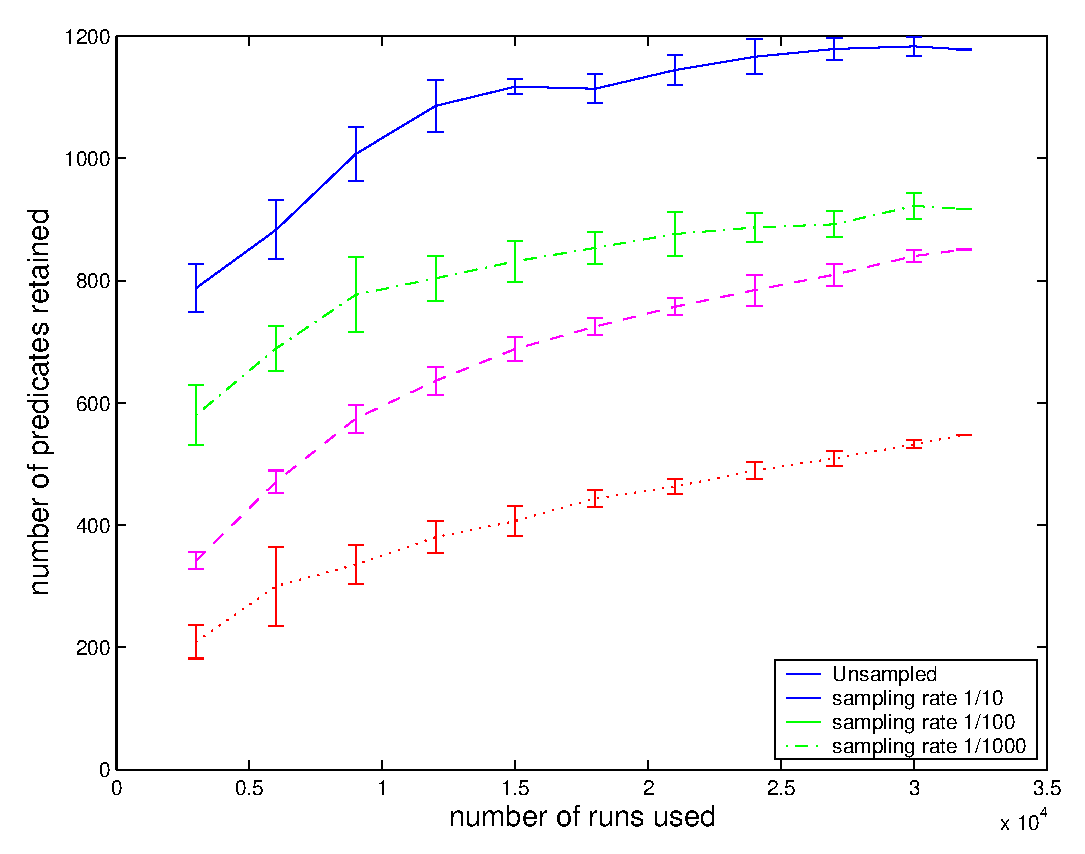
\includegraphics[width=\columnwidth]{predkept3a}
(a) Branches, returns, and scalar-pairs. \\
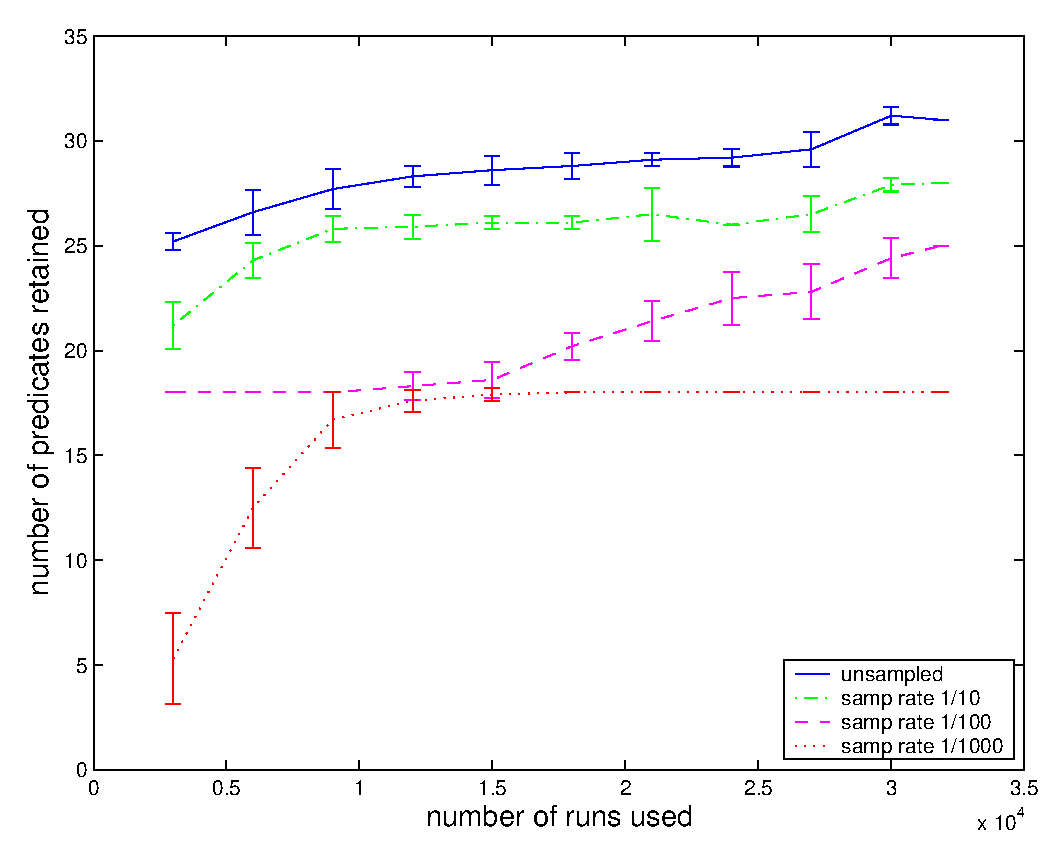
\includegraphics[width=\columnwidth]{predkept3b}
(b) Branches and returns only.
\caption{The effect of sampling and data size on the number of
  predicates selected.}
\label{fig:predkept}
\end{figure}

Two trends are apparent from \Autoref{fig:predkept}.  As one would expect,
the number of retained predicates decreases as the sampling rate decreases,
and increases as more trial runs are included.  If we had an unlimited number
of trial runs, the number of retained predicates at all sampling rates should
approach the result with no sampling.  

Note also that increasing 
the number of trial runs always seems to increase the number of retained 
scalar-pairs predicates, whereas the branch and returns predicates run into 
a plateau at lower sampling rates.  Though there may not be much significance 
in this discovery, we conjecture that it is due to the fact that scalar
pairs predicates are much more often observed than the other two kinds of
predicates.  Therefore determining the importance of scalar pairs predicates
takes much fewer sampled trial runs.

%% As is apparent from the graph, there is much larger variation in the
%% number of selected predicates when we use fewer trial runs.
%% %Using $3000$ trials, at the minimum we
%% %retain $7429$ predicates using unsampled data, $7654$ when sampling
%% %rate is $\nicefrac{1}{10}$, $7347$ at $\nicefrac{1}{100}$, and $6750$
%% %at $\nicefrac{1}{1000}$;
%% As we incorporate more examples of successful and failed \moss\ runs,
%% the variances decrease for all sampling rates, but the means behave
%% somewhat differently.  When the data is not sampled, the average
%% number of selected predicates stays around $8100$ for all data sizes.
%% Sampling adds noise to this procedure.  As we observed previously,
%% a moderate sampling rate tends to drive up the $\increase(\ldots)$ scores, and
%% thus enlarges our set of selected predicates (except when we are using
%% very few trial runs).

%% At the relatively high sampling rate of
%% \nicefrac{1}{10}, there are still enough samples taken at most
%% instrumentation sites, and there is a net increase in the number of
%% selected predicates.  Once the sampling rate shrinks to
%% \nicefrac{1}{100} and below, however, the effect of sparse
%% sampling sets in.  Fewer samples are taken overall on fewer predicates,
%% and as a result, fewer predicates have a nonzero $\increase(\ldots)$ score.
%% Incorporating more runs tends to alleviate the situation; at above
%% 10,000 runs, roughly the same number of predicates are retained for
%% the \nicefrac{1}{100} sampled data as the complete data.  The very
%% sparse sampling rate of \nicefrac{1}{1000}, on the other hand,
%% causes much more change in the final result.  A lot more predicates
%% are eliminated when using fewer trials, and a lot more predicates are
%% retained using more trials.

%% Most of the volatility in the results come from the scalar-pair
%% predicates.  \Autoref{fig:predkept-b} shows the same graph for
%% only the branch and return predicates.  Here, across all data sizes,
%% the number of selected predicates remains roughly constant at each
%% sampling rate.  The complete data is still able to select the fewest
%% number of predicates, with \nicefrac{1}{100} sampled data following
%% close behind.  The \nicefrac{1}{1000} sampled data still produces a
%% net increase in the number of selected predicates.

%% LocalWords:  downsampling lang downsampled predelim predkept
